\clearpage
\begin{flushright}
	\textit{Лекция №20}
	\textit{2015.12.01}
\end{flushright}

Обнаружение тупиков выполняется методом редукции графа (сокращения графа). Сократить дугу можно в том случае, если запрос процесса может быть удовлетворен. В результате редукции могут образоваться изолированные вершины, и если все вершины графа изолированные, то система  не находится в тупике. Если остались не сокращенные вершины, то они в тупике. Мы уже писали три теоремы. Тупик – замкнутая цепь запросов, может возникнуть только в результате запроса. Обнаружение тупиков может представляется в виде матрицы распределения и матрицы запросов. Также необходимо иметь инфо о свободных ресурсах системы (вектор свободных единиц ресурса F)
$F = [\cdots fi \cdots]$, $f_i$ - количество свободных единиц $i$ ресурса. Если просуммировать все выделенные единицы $i$ ресурса и сложить со свободными единицами ресурса, то получим кол-во единиц данного ресурса в системе. 
Первый лобовой алгоритм – метод прямого обнаружения. Просмотр по порядку матрицы запросов, и там где можно, производятся сокращения.
Более эффективный - на анализе векторов. Пусть имеется два вектора C  и  D. 
С <= Д (каждый элемент вектора С меньше или равен вектора Д). Тогда, если i процесс запросил j ресурс и при этом строка запроса i процесса меньше или равна вектору F, то такой зарос может быть удовлетворен. Процесс, запрос которого может быть удовлетворён, может завершиться, и освободить занимаемые им ресурсы, и сократить граф по вершине данного ресурса. 
Более эффективно, если хранить дополнительную информацию о запросе. Для каждого ресурса хранятся запросы, упорядоченные по размеру. Для каждого процесса i, определяется счетчик ожидания, обозначим Wi, этот счетчик содержит число типов ресурсов , которые вызвали блокировку процесса (счетчик отражает число типов ресурсов, на которых процесс заблокирован) Среди заблокированных процессов ищется цикл запросов. 
Алгоритм Бенсусан и Мерфи описан в книге Медника-Донована. В книге – особенности реализации упр. памятью, процессорами, процессами, взаимодействие процессов, проблема тупиков. Книге не устарела, так как архитектура компов – не изменилась.

\begin{figure}[H]
    \centering
    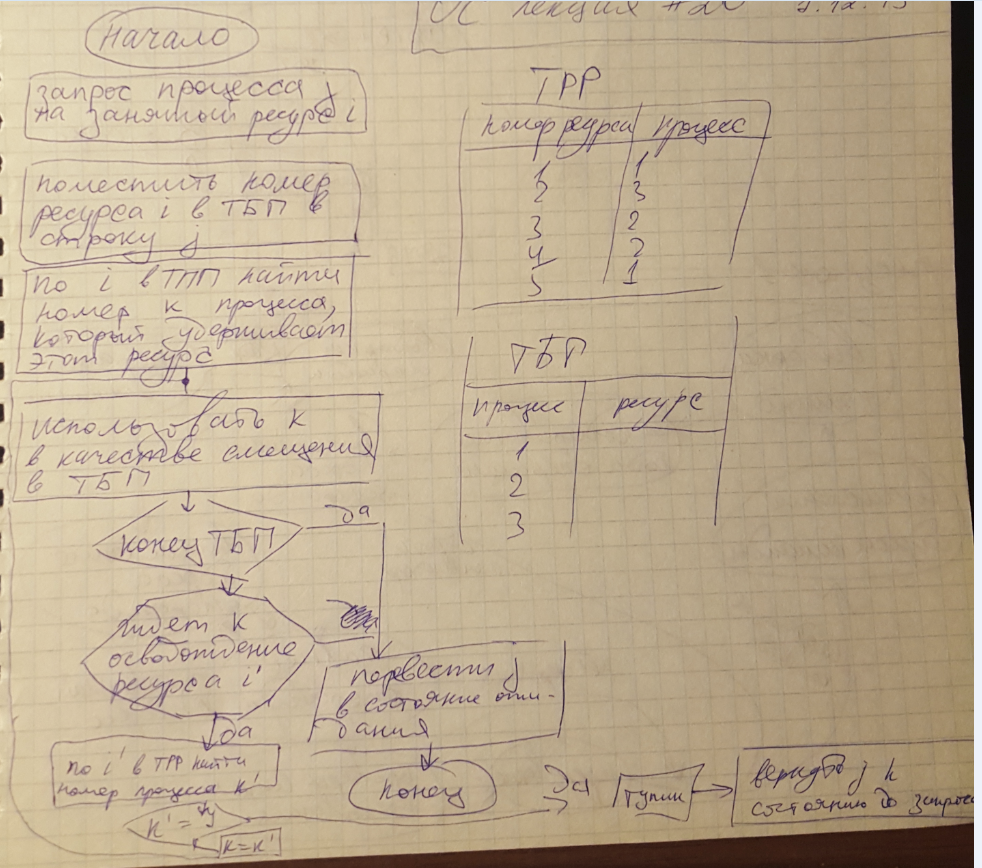
\includegraphics[width=\textwidth]{pic/1.png}
    \caption{pic}
\end{figure}

\begin{figure}[H]
    \centering
    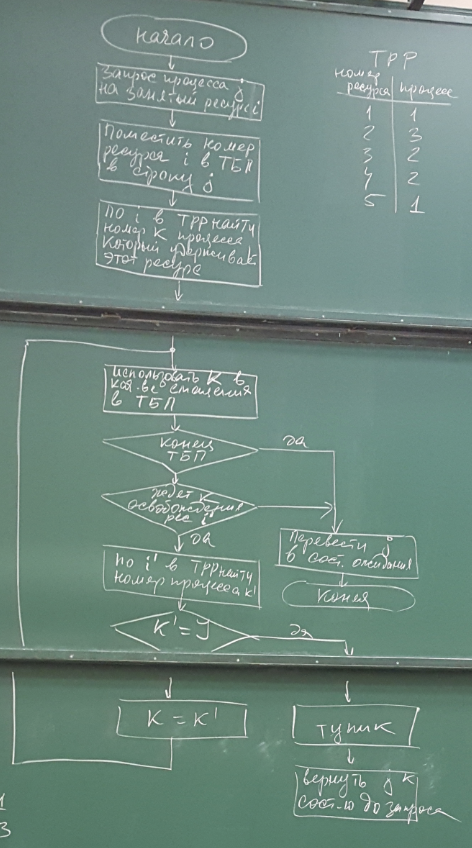
\includegraphics[width=\textwidth]{pic/2.png}
    \caption{pic}
\end{figure}

ТБП – таблица блокированных процессов. ТРР – таблица распределенных ресурсов.

\begin{table}[H]
\caption{tbl}
\begin{tabular}{|l|l|}
1 &  p1 запросил и получил r1\\
\hline
2 &  p2 запросил и получил r3\\
\hline
3 &  p3 запросил и получил r2\\
\hline
4 &  p2 запросил и получил r4\\
\hline
5 &  p1 запросил и получил r5\\
\hline
6 &  p1 запросил и получил r3\\
 & j = 1, i = 3 -> k = 2 \\
 & блокируем процесс 1 на ресурсе 3\\
\hline
7 &  p2 запросил и получил r2\\
 & j = 2, i = 2 -> k = 3\\
 & блокируем процесс 2 на ресурсе 2\\
\hline
8 &  p3 запросил и получил r5\\
 & j = 3, i =5 -> k = 1\\
 & по к в ТБП видимо, что i’ = 3 -> k’ = 2 ->\\
 & k = 2 -> i’ = 2 -> k’ = 3  -> обнаружили замкнутую цепь запросов\\
\end{tabular}
\end{table}

У алгоритма много ограничений. Ресурсы – в единственном экземпляре.
Сток – любая вершина из подмножества процессов, которая не имеет ребер, выходящих из неё. Т.е. процесс получил все ресурсы и у него нет запросов. 
Последовательное исключение ребер, направленных в сток. Если длительное время не выполняются необходимые действия, то можно предположить, что система в тупике. На мейнфрейме такое предположение более реально по сравнению с распределенной системой, так как в РС задержки непредсказуемы.  Если обнаружили, что система в тупике, то выполняются действия, которые мы обсудили. 
Другой подход. Если тупик возник в результате запроса, то можно анализировать состояние системы по ???. 
Для непрерывного обнаружения анализируется каждый запрос. При этом надо проверить, не возникает ли при этом запросе цикл по вершине pi 
Два подхода выхода из тупика:
1. Прекращение выполнения процессов. Приводит к потере проделанной процессами работы.
Определить перечень процессов, попавших в тупик и последовательно завершать их. Освобождаются ресурсы этих процессов. Можно за основу брать приоритет процессов, но со временем он уменьшается, в результате можем завершить процесс, который долго работал и сделал много работы. Другой подход – выключить процесс, который не попали в тупик. 
2. Перехват ресурсов. Тупик возникает в результате запроса на отсутствующий свободный ресурс. Если перехватить нужные ресурсы у других процессов, то их можно выделить тупиковым процессам. Чтобы перехватить ресурс, нужно фиксировать состояния процессов и возвращать какой-то процесс к состоянию до получения конкретного ресурса.
Какие системы вообще не могут попадать в тупик? – реального времени. Это системы, управляющие внешними процессами или объектами. 
Существует два аспекта: надежность и живучесть. Система должна уметь перестраиваться.

\chapter{Архитектура вычислительный систем с точки зрения ядра}
Рассмотрим монолитное и микроядро. 

Существует две структуры ядер:
\begin{enumerate}
    \item Монолитное – программа, имеющая модульную структуру. Т.е. состоит из подпрограмм. Единственным способом, изменить функциональность ядра, это перекомпиляция ядра.
   \item В микроядерной архитектуре все компоненты ОС являются самостоятельными программами и возможно выполняются в разных адресных пространствах. Взаимодействие между такими модулями ОС выполняется по модели клиент – сервер. Взаимодействие осуществляется путем передачи/приема сообщений. Основная функция ядра – осуществление взаимодействия процессов с помощью сообщений.
\end{enumerate} 
